% !Mode:: "TeX:UTF-8"
% !TEX root = ..\Literature_Translation.tex
\kchapter{现行调度方法}
下面将引入相关符号,并对案例中的工厂所运用的现行调度方法进行描述。
\ksection{符合说明与相关假设}
为了方便问题描述,符号说明如下:%\\[5pt]

\begin{supertabular}{ll}
$j$ & 作业标记 \\
$i$ & 批次标记\\
$r$ & 批次中的位置标记\\
$b$ & 工段中的批数,$b\geqslant2$\\
$c$ & 工段1的批量\\
$J$ & 需要调度的作业集合,$J=\{1,2,...,n\}$\\
$p_{aj}$ & $J_j$在工段$a$的单件处理时间,$p_{aj}=p_a$\\
$p_{1j}$ & $J_j$在工段1的处理时间,$p_{1j}=p_1$\\
$p_{2j}$ & $J_j$在工段1的处理时间\\
$s_a$ & 在工段1的作业换线时间\\
$s_b$ & 在工段2的批次换线时间\\
$s_{f1}$ & 在工段1的产品簇换线时间\\
$s_{f2}$ & 在工段2的产品簇换线时间\\
$f_j$ & $J_j$的产品簇,$f_j=1,2,3,4$\\
$f_{1,[i,r]}$ & 在工段1中安排在第$r$批次作业$[i,r]$的产品簇 \\
$f_{2,[j]}$ & 在工段2中安排在第$j$批次$J_{[j]}$的产品簇 \\
$k_{1,[i,r]}$ & \begin{numcases}{=}
{\liuhao 0 }&{\liuhao 在工段1,如果作业$[i,r]$和它的前继作业同属一个产品簇}\notag\\
{\liuhao 1 }&{\liuhao 其他情况} \notag
\end{numcases}\\[5pt]
$k_{2,[j]}$ & \begin{numcases}{=}
{\liuhao 0 }&{\liuhao 在工段2,如果$J_[j]$和它的前继作业同属一个产品簇}\notag\\
{\liuhao 1 }&{\liuhao 其他情况} \notag
\end{numcases}\\
$S$ & 已调度的作业集合\\
$S_U$ & 未调度作业集合\\
$B$ & 已调度批集合\\
$B_i$ & 工段1的第$i$批,$B_i\subset B$\\
$p_1(B_i)$ & 工段1的$B_i$处理时间\\
$D_j$ & $J_j$的交货期\\
$d_j$ & $J_j$的工期\\
$d_{[j]}$ & $J_{[j]}$在工段2的工期\\
$C_{1,[i]}$ & 批$i$在工段1的完工时间\\
$C_{2,[j]}$ & $J_{[j]}$在工段2的完工时间\\
$T_j$ & $J_{[j]}$的滞后时间\\[10pt]
%$$ & \\
\end{supertabular}
%\end{center}

下面是该问题的相关假设:
\begin{itemize}
\itemsep=0pt\parskip=0pt
\item 所有作业在0时刻皆未被占用;
\item 作业总量可被批量大小$c$整除,即$n=b\times c$;
\item 批次中的作业需在工段1处理完该批后方可开始工段2的处理;
\item 工段1中处理单件需要考虑作业换线时间$s_a$;
\item 工段1上的批量处理需要考虑批量换线时间$s_b$;
\item 新产品簇在工段1上加工前需要考虑产品簇换线时间$s_{f1}$;
\item 新产品簇在工段2上加工前需要考虑产品簇换线时间$s_{f2}$;
\item 事先已获得固定的处理时间、换线时间和交付期。
\end{itemize}
\ksection{生产制造过程}
为了简化流程和扩大生产能力,所有零件、组装子件全部外包给资深的合作伙伴或零售商。因此,该生产系统可以被构建成一个两阶段装配流水车间:
\begin{inparaenum}[(1)]
\item 一个组装工段,用来将零部件、模块等组装成框架;
\item 一个集成工段,应用了机械电子工程(M\&E)的集成手段。
\end{inparaenum}
应用模块化设计和标准化以允许所有产品共享同条生产线,并且有着相同的生产时间。如此一来,所有产品都可由11个子系统构成,如\reft{tab:11+4}所示。
\begin{table}[h]
  \centering\xiaowu
  \caption{11个子系统和4个作业块(A,B,C,D)}
    \begin{tabular}{llllll}
    \toprule
    \multicolumn{2}{c}{前部} & \multicolumn{2}{c}{中部} & \multicolumn{2}{c}{后部} \\
    \midrule
    A-1   & 推辊机   & B-1   & 水平电子码(EPC)机 & D-1   & 袋酱机 \\
    A-2   & 张力锟机  & B-2   & 垂直电子码(EPC)机 & D-2   & 冲孔机 \\
    A-3   & 压袋机   & B-3   & 封刀机   & D-3   & 输送机 \\
    A-4   & 送料机   & C-1   & 摇摆系统  &       &  \\
    \bottomrule
    \end{tabular}%
  \label{tab:11+4}%
\end{table}%
需要考虑各子系统的负荷和操作进程,以平衡产线和缩短完工时间(Nearchou,2011)。所有的操作被分解成4个操作块(A,B,C,D),并且分别指派给4位一组中的熟练工。这4位工人将框架和底架移至工段1的同一个区域以开始作业的操作,同时他们需要准备好操作的所需部件和工具。而后,他们便开始在各自的操作块中进行组装。
由于空间限制,组装操作很容易产生人员间的干涉,并会由此产生潜在的等待时间,这常常会导致生产瓶颈。
每当作业在工段1的组装操作结束,便会转移到工段2,由2位该组的熟练工继续作业。他们运用机电集成技术,包括伺服或计算机系统安装、参数设置、调试等。之后,完成的作业被移至成品区。

\ksection{换线时间和产品簇}
大多数有关调度的研究将换线时间看做是可忽略或者将其算作处理时间的一部分(Logendran,2005;Allahverdi,1999),但是在此案例中,换线时间是很重要的,不得不考虑。此处,换线时间可以归为两类:
\begin{inparaenum}
\item 作业换线,作为工作准备,将所有要处理作业的零部件置好;
\item 产品簇换线,用于获得工具、调整工装夹具、检查不同产品簇的需要加工零部件(Eren,2007)。
\end{inparaenum}
工段1在操作开始前,需要一个作业换线时间$s_a$,而当开始第1个作业或切换产品簇的时候,在两个工段都需要考虑产品簇换线时间$s_{j1}$和$s_{j2}$。简化起见,我们假设这些都是常数,即$s_a=5.2\ h$,$s_{f1}=3.2\ h$,$s_{f2}=1.6\ h$。如\reft{tab:2yearproduction}所示,现有超过10个模块在案例工厂加工,并且这些作业可以根据模块属性群组为4个产品簇($f_1\sim f_4$)。需要注意作业处理时间不包括换线时间$s_a$,因为它需要和批次换线时间换线时间$s_b$作比较。
\begin{table}[htbp]
  \centering\xiaowu
  \caption{近两年作业的模块和产品簇的产量}
    \begin{tabular}{lrcccc}
    \toprule
    \multicolumn{2}{c}{模块} & \multicolumn{2}{c}{数量} & \multicolumn{2}{c}{处理时间(h)} \\
    \midrule
    \multicolumn{1}{l}{编号} & \multicolumn{1}{c}{产品簇 } & 2007  & 2008  & $p_1/1$位工人 & $p_2/2$位工人 \\
    \midrule
    900BR & \multicolumn{1}{c}{$f_1$} & 26    & 15    & 24    & 16 \\
    1000DT & \multicolumn{1}{c}{$f_1$} & 30    & 46    & 24    & 16 \\
    800ST2 & \multicolumn{1}{c}{$f_2$} & 44    & 51    & 24    & 12 \\
    1100ST3 & \multicolumn{1}{c}{$f_2$} & 18    & 11    & 24    & 12 \\
    1000TT & \multicolumn{1}{c}{$f_3$} & 43    & 30    & 24    & 8 \\
    800TT & \multicolumn{1}{c}{$f_3$} & 37    & 31    & 24    & 8 \\
    1000VV & \multicolumn{1}{c}{$f_4$} & 21    & 47    & 24    & 10 \\
    其他 & \multicolumn{1}{c}{$f_4$} & 49    & 67    & 24    & 10 \\
    \multicolumn{2}{c}{平均值(每月)} & 22.33 & 24.83 & -     & - \\
    \bottomrule
    \end{tabular}%
  \label{tab:2yearproduction}%
\end{table}%

\ksection{目标函数}
如引言所述,用制造期、完工时间和、滞后时间和等多目标加权求和可以更好地展现该问题,即:
\[Z=\alpha C_{\max}+\beta\sum_{j=1}^n C_{2,[j]}+\gamma\sum_{j=1}^n T_j
\]
式中的$\alpha,\beta,\gamma$位非负权重系数,可以用下面的法则确定:
\begin{compactenum}[(1)]
\item $C_{\max}$和$\sum C_{2,[j]}$不一定有相同的值域。为了减小差异,可以采用Framinan(2002)提出的调节程序。先假设一项有n个独立作业工作的期望完成时间为$C_{\max}/2$,因此$nC_{\max}\approx\sum C_{2,[j]}$,相当于将$C_{\max}$和$\sum C_{2,[j]}$与$n/2$和$1$分别相乘。
\item 实践中,权重系数的确定很大程度上取决于决策者(Taboada 和Coit,2008)。在案例的工厂中,完工时间和可以帮助评估及时交付情况,而滞后时间和主要作为超时加班计划的目的。一版安排完工时间和与滞后时间和为制造期的2倍。所以,$C_{\max},\sum C_{2,[j]}$和$\sum T_j$需分别再乘以1,2,2。如$n=12$,则权重为$(\alpha,\beta,\gamma)=(6,2,2)=(0.6,0.2,0.2)$。
\end{compactenum}
\ksection{现行调度方法}
现行的调度方法工作流程如\reff{fig:csf}所示。
\begin{figure}[h]
\centering
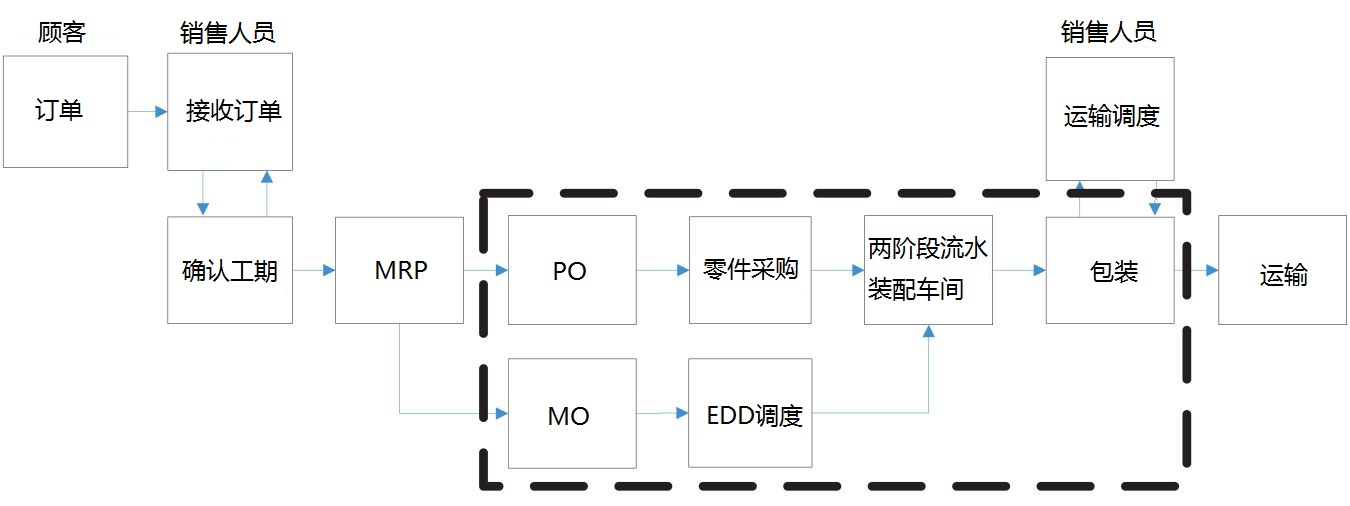
\includegraphics[width=16cm]{current_flow.jpg}
\caption{现行调度方法工作流程\label{fig:csf}}
\end{figure}
生产管理员确认了交付期后,销售人员接受顾客的订单并将订单通知发给生产管理员。当订单通知下达车间时,MRP 中心发布采购订单(PO)和制造单(MO)。通常工期以周计算,要比交付期$(D_j)$提前$5\ days\times 8\ h=40\ h$,即$d_j=D_j-40$。所有的采购订单需以PO 的基础立即呈给供应商,同时,生产调度需立即按MO 的基础制定。目前,作业的顺序按EDD 分派规则制定,并且单件流(Li 和Rong,2009)将在两个工段按相同顺序执行。

当换线时间等于0时,EDD 规则是最小化最大延迟的最优解(Baker 和Magazine,2000)。然而,现今的车间中,许多作业换线时间和产品簇换线时间会在单件流的情况下产生,所以EDD 规则通常会得到较大的完工时间。进一步说,在单件流情况下,4为工人同时在有限的空间内操作(见\reff{fig:cwf}),时常会相互干涉,产生可相当可观的闲置时间,使得处理时间从$p_a=24\ h/4=6\ h$变为$p_a=9\ h$(见\reft{tab:2yearproduction})。因此,现行调度方法将产生下列问题:
\begin{compactenum}[(1)]
\item 单件流会导致物料短缺,产生不能满足调度的处理困难;
\item 频繁换线和闲置使得流程时间变长和更多的超时加班;
\item 由于按期完成率低,不能处理紧急订单。
\end{compactenum}

为了解决这些问题,我们提出了作业划分和批量作业的的策略,将在接下来的章节里讨论。